% \noindent\begin{figure}[htb]
% \centering
% \begin{minipage}[t]{0.48\textwidth}
% \includegraphics[width=1\textwidth]{images/konigsberg.jpg}
% \end{minipage}\begin{minipage}[b]{0.48\textwidth}
% \centering
% \begin{tikzpicture}
%     \tikzset{LabelStyle/.style= {draw}}
%     \GraphInit[vstyle=Normal]
%     \node[VertexStyle](A){a};
%     \node[VertexStyle,right=of A](B){b};
%     \node[VertexStyle,right=of B](C){c};
%     \node[VertexStyle,above= 1.2cm of B](D){d};
%     \draw[EdgeStyle](B) to node[LabelStyle]{} (D);
%     \tikzset{EdgeStyle/.append style = {bend left}}
%     \draw[EdgeStyle](A) to node[LabelStyle]{} (B);
%     \draw[EdgeStyle](B) to node[LabelStyle]{} (A);
%     \draw[EdgeStyle](B) to node[LabelStyle]{} (C);
%     \draw[EdgeStyle](C) to node[LabelStyle]{} (B);
%     \draw[EdgeStyle](A) to node[LabelStyle]{} (D);
%     \draw[EdgeStyle](D) to node[LabelStyle]{} (C);
% \end{tikzpicture}
% \end{minipage}
% \caption*{\textsf{The city of K{\"o}nigsberg in an old postcard with its graph-theoretical representation, where the bridges are the edges of the graph and the city parts are represented by nodes.
% This city inspired Euler to start graph theory.}}
% \end{figure}

%%%%%%%%% INTRO GENERALE COMPLEX NETWORKS
%\section{Complex networks science and the brain}\label{sec:complexnetworksciencebrain}

\section{The rise of network neuroscience}
Starting from 19th century’s neuron doctrine, the brain is described as an incredibly complex system of intercommunicating elements, the neurons, intertwined with other cells that support neuronal activity.

The dynamical processes running on the biological substrate of neurons are the basis of information processing that gives rise to cognitive and psychological processes, from the perception of the external environment to the representation of mental states and emotions.
Neuroscience tackles the investigation of the brain, the most complex organ in nature, at different scales.
Molecular and cellular neuroscience focus on the finest level of workings of the nervous system cells.
At this scale, molecular biology and genetics are used to address the study of very small populations of neurons.

At larger scales, hundreds or thousands of neurons are involved and a more comprehensive approach is needed.
The view must shift from the microscopic level to the so-called systems neuroscience, which deals with widespread networks of neurons, dubbed neuronal circuits.

System neuroscience studies how these large-scale circuits form and evolve during  development, how they produce basic processes like reflexes, motor coordination, circadian rhythms and, ultimately, how they give rise to behavioural and different internal states like motivation, emotions, and cognition.
Hence, an extension of system neuroscience from the study of small groups of neurons to the whole brain requires radically different tools, both computational and experimental.
Very small scale neuronal circuits can be studied by mathematically accurate models.
The typical size of the smallest identified functional unit, the cortical column, is around hundred thousand neurons and, already at that level, many hypotheses are required to approximately reproduce the electrical and chemical activity of neurons, at the point that a comprehensive differential equations model of cortical columns is still lacking.

Yet, a large-scale understanding of the incredibly complicated network of all the neurons in the human brain, the \emph{human connectome}, remains a challenging target to be reached in the future~\cite{amunts2016}.
This scientific, technological and cultural challenge is named after the term \emph{connectomics}, a word coined at the beginning of this decade by Giulio Tononi and Olaf Sporns~\cite{sporns2005}.
Its most ambitious aim is to map all the connections in the brain at different scales of resolution, deep down to the synaptic level.
Whether this will help answer some of the deepest questions about the human brain, it is not entirely known and still a topic of hot debate in the scientific community.

The science of brain connectivity takes advantage of well-consolidated technologies for looking at the brain at work.
These non-invasive methods of analysis of brain functions include neuroimaging techniques like magnetic resonance imaging (MRI), electroencephalography (EEG) and transcranial magnetic stimulation (TMS).
Among these modalities, MRI has emerged as a dominant non-invasive imaging method because it enables the investigation of both brain structure and function with a good compromise in terms of spatial and temporal resolution.

At the morphological level, MRI provides a comprehensive view of the brain, as it can identify the white matter fiber pathways connecting gray matter regions otherwise impossible to obtain in-vivo.
The pattern of white matter fibers is often named after the term \emph{structural connectivity} as it relates to the morphological features of the brain connections.
Structural networks correspond to a pattern of anatomical connections, summarizing bundles of axons connecting different brain regions.
Borrowing ideas from the electronics, structural connectivity may be interpreted as the electrical wiring of the different parts of a processor.
Although useful, the wiring diagram of the brain is only a starting point for making hypotheses about the brain at work; indeed it cannot reveal how neurons behave in real-time, nor does it account for the yet unknown regulatory mechanisms that neurons exert on each other.
Unfortunately, these dynamics are and remain partially unpredictable, despite many notable and useful attempts~\cite{deco2008}, as also the synaptic weights are changing dynamically due to synaptic plasticity.

The discovery of the BOLD effect in the 90's by Ogawa~\cite{ogawa1990}, led to functional MRI, a method to spatially map activity in the whole brain.
Considered over the large scale, the BOLD response is descriptive of the temporal metabolic demands of large groups of cortical and subcortical structures, a quantity strictly related to the electrical activity of neurons~\cite{logothetis2001}.
This tool helped scientists to unveil another pattern of connectivity that exists in the brain. \emph{Functional connectivity} examines functional associations between temporal fluctuations of neuronal activities from different brain regions~\cite{biswal1995}.
Activation maps have been estimated for almost every kind of cognitive task and collected in publicly available datasets, like the BrainMap database~\cite{fox2002}, the Neurovault repository~\cite{gorgolewski2015} and the UCLA multimodal connectivity database~\cite{brown2012}.
 %Specifically fMRI functional connectivity focuses on the underlying physiological dynamics giving rise to changes in blood oxygenation.
%Since its inception, the evolution of technologies in MRI, lead to functional MRI (fMRI), a way to spatially map temporal changes of oxygenated blood concentration in the whole brain, the so-called BOLD signal.
%Throughout the years, fMRI helped neuroscientists and neurologists to enrich the knowledge of the fundamental aspects of the normal brain functional organization, but as every technique also has its limitations~\cite{logothetis2008}.
% and yields precious information about the brain not only on its surface but also in other deeper regions, otherwise difficult to reach.
In contrast to structural connectivity, functional connectivity results from estimates of statistical dependencies between neuronal or regional time courses.
Functional networks may vary over time, unlike structural networks which are stable over long time scales. For instance, electrical patterns of cortical activity may rearrange over time-scales of milliseconds, in contrast to structural ones, involved in processes like nervous system development, learning and aging.
Furthermore, the temporal evolution of functional networks is variable as it exhibits spontaneous changes during rest and characteristic modulations for different task conditions~\cite{honey2007,hutchison2013}.
%Importantly, functional connectivity does not express any causal effects between brain regions, as it's only informative of their statistical dependence.

%Together with the lesion studies accumulated over two centuries, they greatly increased the awareness of many aspects of brain organization.
When cognitively at rest, the brain engages in a characteristic pattern of dynamic neural activity and most brain regions show spontaneous oscillations in the BOLD signal~\cite{biswal1995,raichle2001,gusnard2001}.
Interestingly, this background activity dubbed \emph{resting-state connectivity}, is not extinguished but only attenuated during tasks~\cite{fransson2006}, making evident its importance in response to changes in the external demands.
The fluctuations of resting-state connectivity typically exhibit the highest correlation at low temporal frequencies (<0.1 Hz) and can be observed during alertness~\cite{fox2006}, sleep~\cite{horovitz2009}, light sedation~\cite{greicius2008} and general anaesthesia~\cite{martuzzi2010}.
The structure of temporal correlations of the BOLD signals defines a network over spatially remote, intersecting brain regions. 
Interestingly, these networks are altered in neuropsychiatric diseases like autism~\cite{rudie2013} and schizophrenia~\cite{vandenheuvel2014}.
The extent of these alterations may be an hallmark for possible diagnoses of brain disease.

Complex network science provides a framework to study the structure of functional connectivity networks and to assess alterations induced by pathological conditions~\cite{bullmore2009,stam2014,crossley2014,fornito2015}.
%Among the many methods that are available to detect such pathological alterations, one of the most important is the possibility to quantify the modifications of the resting state networks in the abnormal brain using the theoretical framework of complex networks science~\cite{sporns2000,sporns2002,sporns2004,bullmore2009,stam2014}.

%Complex network science offers the best tools to assess the topology and organization of brain connectivity networks, as well as powerful means to establish, in a completely data-driven manner, diagnoses of common neurological diseases offering the possibility to design lines of intervention and prevention.
%In the framework of complex networks science, the brain is seen as a system whose fundamental units are the brain regions at different scales, interconnected by a number of links, describing the strength of inter-regional coordination.

%%%%%%%%%%%%%%%%%%%% RIPRESO DA INTRODUZIONE
The methods of network theory date back to the problem of K{\"o}nigsberg bridges, in 1735, when the famous mathematician Leonhard Euler was faced with the problem of finding a path through the city that would cross all the seven bridges just once.
The knowledge accumulated since then forms the basis of modern graph theory.
In totally general settings, simple graphs are usually defined as a set of nodes,  connected by a set of links, denoting the strength of the relation between pairs of nodes.
Graphs can be used to represent any type of relation between interacting elements and the idea that graph-theory can be applied to brain networks has been pioneered starting from the middle nineties defining a new specialization of systems biology, dubbed \emph{network neuroscience}.

The network neuroscience relies upon the treatment of the brain as a graph, whose nodes are indicative of particular brain regions connected by links representing  the strength of their mutual interactions.
The classical general pipeline for the definition of a brain graph is given in Figure~\ref{fig:bullmore2009pipeline}.
In this framework, the modelling of the brain in terms of graphs starts from the definition of its nodes~\cite{stanley2013}.
These can be defined as anatomically or functionally defined regions~\cite{vandenheuvel2010}.
A clear delineation of network nodes is one of the first steps in the whole pipeline of the graph-theoretical analyses and is highly important for the subsequent analyses~\cite{stanley2013}.
The second step in the definition of a brain network is an estimate of the continuous association between nodes: the links of the graph indeed measure the interregional coordination or similarity between nodes~\cite{pereda2005a}.
To be more specific, in the case of fMRI studies of resting state functional connectivity, link weights are defined as interregional temporal correlations in the fluctuations of the BOLD signals, and the resulting graph can be represented by a square matrix (adjacency matrix) where the strongest correlations indicate the presence of a link between any two specific areas.
In other applications, like Diffusion Tensor Imaging, a technique that is able to show the effective directions of nervous fibers traits in the brain, one can define links whose strength is directly proportional to the number of white matter tracts connecting any two regions.
In addition, brain networks have also been defined on the basis of inter-subject anatomical covariance~\cite{evans2013,he2007}, co-activation of different brain regions across individuals subjected to experimental tasks~\cite{crossley2013a}, pharmacological challenges~\cite{schwarz2007,schwarz2008} or spectral coherence of EEG electrical time-courses~\cite{pereda2005a}.
All of these networks are ``weighted'' by definition, i.e. their links are associated with real numbers representing a measure of the strength of pairwise interactions between nodes.

%% FIGURA BULLMORE
\begin{figure}[htb!]
\centering
\includegraphics[width=1.0\textwidth]{images/bullmore_2009_pipeline.pdf}
\caption{Structural and functional brain networks can be explored using graph theory through four steps.
Adapted from~\cite{bullmore2009}.}
\label{fig:bullmore2009pipeline}
\end{figure}

The rise of the network neuroscience in the last decade has been driven by the evidence that almost independently from how the networks links are defined, brain networks share some common features at many spatial and temporal scales.

For example, they exhibit the \emph{small-world} property~\cite{watts1998,sporns2002,sporns2004a}, whereby most nodes in a graph can be reached from any other node in just a few hops.
Small-worldness in brain networks~\cite{vandenheuvel2008} has been found to positively correlate with higher IQ in humans~\cite{vandenheuvel2009}, suggesting that human intellectual performance may be related to how efficiently our brain integrates information between multiple brain regions.

Other measures have been correlated with phenotypical and structural characteristics.
\emph{Rich-clubs} are subsets of highly connected nodes who are also highly connected to each other, forming a communication backbone.
It has been hypothesized, that rich clubs might be valuable in supporting high-level and more cognitively advanced forms of information processing~\cite{collin2014}.
Moreover, it's thought that the presence of a rich club increases the diversity of the functional repertoire over and above the effects produced by scale-freeness alone~\cite{senden2014}, a property of a network of being self-similar at different scales.
Forms of rich-club organization have been observed in cats, macaque and humans~\cite{vandenheuvel2011,harriger2012,dereus2013a,collin2014}, comprising portions of prefrontal, parietal, temporal and insular cortex.
Rich club nodes and edges participate in a large number of short paths across the network, contributing disproportionately to global communication.

From the functional point of view, central hubs of rich clubs are concentrated in heteromodal association cortices, areas that receive input from multiple unimodal sensory association areas and/or other heteromodal cortices~\cite{sporns2007,power2013,kandel2013}.
Contrarily, primary sensory cortices have low topological centrality and degree~\cite{vandenheuvel2011,zamora-lopez2010,harriger2012}.
Damage to primary sensory areas only affects them locally, while perturbation to the rich-club backbone has diffuse and severe effects on the whole network architecture~\cite{honey2008,ball2014}.
Abnormal rich-club connectivity is hypothesized to be related to familial vulnerability for schizophrenia~\cite{collin2014impaired} and other diseases as well.

More generally, network neuroscience has matured the ability to map alterations at the level of structural or functional connectome and may be useful for predicting and generating hypotheses about underlying pathophysiological mechanisms of disease.
%Clinically useful predictions are now being made on the basis of network indicators, viewed as biomarkers of brain alterations~\cite{fornito2015}.
%Hence, if only a systematic biological study of the nervous system can detail the etiology of neurological diseases, their observable symptoms often result in a partial or total reorganization of the functional and structural architecture of the brain.
To this end, the definition and validation of data-driven biomarkers based on graph-theoretical observations of the effects of brain diseases is a highly desirable objective.

\section{Brain networks at the mesoscale}
Many natural and artificial networks display a modular organization, i.e. nodes group together in some kind of \emph{clusters}, resulting in a particular mesoscopic structure.
At this level of mesoscale organization, the topological properties of nodes are more dependent on their neighbourhood than on the rest of the graph.
When the structure tends to group nodes with similar properties, the mesoscale structure is called \emph{assortative}.
Graphs with an assortative structure consist of tightly connected groups of nodes that are themselves loosely connected with other groups.
These groups are therefore dubbed as \emph{communities}.

The organization into communities is one of the most studied properties of networks and a large amount of literature has grown on the topic, as reviewed in~\cite{fortunato2010}.
The problem of detecting the communities, \emph{community detection} or \emph{graph-partitioning} in the computer-science jargon, is of high theoretical and practical importance.
From the theoretic point of view, communities are representative of the generative probabilistic model underlying the formation of links~\cite{karrer2011} and tell much about the statistical properties of networks.
On the other side, practical applications of community detection are fundamental not only in neuroscience but also in sociology, computer science, biology and many other fields.
Modules derive from a decomposition of the network into subcomponents that are internally strongly coupled but externally only weakly coupled.
The property of a system of being modular or \emph{nearly-decomposable}, as already noted by Nobel prize laureate Herbert Simon~\cite{simon1991}, helps any system to resist external perturbations by separating different functions into topologically distinct part of the system.
Near decomposability is in many respects a hallmark of complexity in natural systems\cite{simon1991}.

Strong experimental evidence shows that the nervous system in animals and humans, from the neuronal level up to macroscopic scale, displays an organization that favours the exchange of information over a communication backbone supported by well-connected areas, the connector hubs of the network~\cite{dereus2013a}, responsible in turn for sending information to local processors, identified as the communities or modules~\cite{vandenheuvel2013a}.
Functional brain networks of humans and other animals, consist of connected subnetworks (or modules) associated with cognitive functions, of vital importance for the daily life and the interaction in the environment.
The modular organization is exhibited hierarchically at different scales, with modules inside modules.
Within this architecture that confers robustness and adaptability to the network~\cite{meunier2010}, information flows from lower level sensory cortices to higher multimodal and associative cortices~\cite{mumford1992}, thus being refined and filtered in its content at multiple stages of elaboration.
The specialized stages of neural information processing are the regions of \emph{functional segregation}, a common feature at multiple scales in the brain, from the neuronal networks to macroscopic anatomically defined regions.
From the functional point of view, segregation is meant as the statistical dependence of processing elements within the same region~\cite{tononi1994}.
\emph{Functional integration} instead is defined as significant deviation from independence of large subsystems, and is typically realized through synchronization processes that increase the statistical dependence between functional modules, a mechanism required to access widely distributed resources, needed for a coherent behaviour~\cite{tononi1998}.
A delicate balance between functional integration and segregation is realized at the edge of metastability as cortical areas are neither fully synchronized nor full desynchronized~\cite{friston1997}.


When the subtle balance between functional integration and segregation is altered, like in pathological states or for external insults, the brain responds in an adaptive manner, in order to maintain homoeostasis, where possible. The mechanisms of homoeostasis adopted are compensation, degeneracy and redundancy~\cite{fornito2015}.
Through compensation, extra neural resources are recruited to maintain normal function and thanks to neural degeneracy and redundancy~\cite{tononi1999}, it is possible for distinct regions to carry out the same function, to some extent.
When these compensatory mechanisms set in after homoeostatic perturbations, the result is a reorganization of the brain structure, involving changes in its network properties.
Among the network level changes observed after specific alterations, those relative to the brain modular structure can be investigated within the framework of complex networks science~\cite{alexander-bloch2010,alexander-bloch2012,meunier2009}.

\begin{figure}[htb!]
\centering
\hfill\includegraphics[height=0.25\textwidth]{images/brain_network_basics.pdf}\hfill
\includegraphics[height=0.25\textwidth]{images/brain_network_communities.pdf}\hfill
\caption{Meaning of communities, hubs and connectors of a brain network, depicted in an artistic view. Adapted from~\cite{sporns2016}.}
\label{fig:brain_network_communities}
\end{figure}

%This kind of structure implies that modules of heterogeneous size are present at the same time in the brain networks and that an efficient method to detect the presence of large and small modules at the same time together is in order.

Using the tools of complex network science, the evaluation of the modular structure of FC networks is cast to the problem of community detection in graphs, i.e. the problem of identifying independent groups of brain regions that exhibit strong interconnection between each other but that are weakly connected to other modules.

%% COMMENTATO DA ANGELO
% With the graph partitioned into smaller groups (or communities) of functionally connected modules, it is simpler to quantify the effect of the disease on the partitioning, as well as the areas involved in such reorganization and the role of the single nodes inside their modules.
% Indeed, an important factor when considering the effects of external perturbations on brain functioning is the degeneracy (or redundancy) of network nodes across their modules.
% Areas that are buried inside a dense module have high degeneracy, as removal of a vertex is unlikely to affect the communications between the others.
% COMMENTATO Generally speaking, poorer prognoses are registered when the interested area of the insult has low degeneracy, i.e. only that area is deputed to a particular region such that no other area may compensate.
%Severe impairments of neurocognitive functions are associated with damages to highly central nodes, as depicted qualitatively in Figure~\ref{fig:prognosis_centrality}.
% \begin{figure}[htb!]
% \centering
% \includegraphics[width=0.75\textwidth]{images/prognosis.pdf}
% \caption{Hypothetical relation between centrality of node subjected to an pathological insult, its degeneracy and the expected functional impairment. Adapted from~\cite{fornito2015}.}
% \label{fig:prognosis_centrality}
% \end{figure}

%%%%%%%%%%%% PARTE COMMUNITY DETECTION %%%%%%%%%%%%%%%%%%%%
Several methods have been proposed to resolve the community structure of complex networks~\cite{fortunato2010,lancichinetti2009,fortunato2016}.
Many of these methods involve the definition of a fitness function that assigns positive or negative scores to edges connecting nodes within or outside the same community, and heuristics to find the optimal partition of the network that maximizes this fitness function.
Among all the methods, the most popular approach is Newman's ``Modularity maximization'' and variations thereof~\cite{newman2006}.
Following the first demonstration by~\cite{schwarz2008}, partitioning of brain networks using Newman's Modularity has been widely applied to assess the brain modular structure.
Despite its wide usage and merits, Newman's Modularity is characterized by some important limitations as it may fail to detect modules smaller than a certain scale determined by the network size, resulting in a few, relatively uniform modules of almost the same dimension.
This general behaviour, not unique to Newman's approach, is pervasive in community detection and is dubbed as \emph{resolution-limit}~\cite{fortunato2007}.

% COMMENTATO DA ANGELO The problems and drawbacks resulting from the resolution limit passed largely unnoticed in the neuroscience literature of the last years as most scientists used Newman's Modularity.
% COMMENTATO DA ANGELO This barrier has its roots in the theoretical foundations of community detection and practically implies that the detection of brain modules smaller than a scale determined by the size of the total network is very difficult, or in the worst case, even impossible.
As a consequence, even unambiguously defined modules, like almost complete sub-graphs or even cliques\footnote{Graphs where all nodes to connect to all nodes}, may be unduly merged into larger communities when they are too small compared to the size of the network.
This limit hampers the ability to detect small-scale structures of functionally correlated brain areas and to notice alterations in connectivity between subjects or groups of subjects. Hence, it may have prevented detection of alterations in the modular structure of brain connectivity in patients affected by various neuropsychiatric disorders
% Such limit is therefore of impediment to an implementation of a clinical-level biomarker of brain disease.
Hence, the resolution limit represents a critical shortcoming for the study of brain networks and is likely to have affected many of the studies reported in the literature.
% TROPPO SPECIFICO A QUESTO LIVELLO
%Moreover, it has been shown that an adjustable resolution parameter may reduce the tendency to merge small clusters, but only at the cost of unduly splitting large clusters~\cite{lancichinetti2011}. Adjustment of the resolution parameter is an attempt to balance these two biases, but multi-resolution methods fail to recover community structures comprising heterogeneous distributions of cluster sizes~\cite{lancichinetti2011}.

In the present work I have developed an approach that has been valuable in detecting communities in brain networks beyond the resolution limit. The following sections of this introductory chapter guide the reader into the complex networks science, by first giving an overview of the mathematical terminology and methodological concepts.
In the second chapter, the experimental evidence of the modular structure of brain connectivity is reviewed, together with the methods to disentangle the mesoscopic structure of complex systems. In particular, sections~\ref{sec:resolutionlimit} and~\ref{sec:degeneracy} consider the problem of the resolution limit and degeneracy of Newman Modularity.
A new approach dubbed Surprise, that overcomes the limitations imposed by the resolution limit and degeneracy, is described in the chapter~\ref{chap:beyondresolutionlimit}. Throughout chapter~\ref{chap:beyondresolutionlimit}, the problems imposed by the resolution limit and degeneracy are analysed for Surprise and its weighted counterpart, Asymptotical Surprise. The characteristics of the two methods are discussed, together with an efficient algorithm aimed at their optimization.
The application of Surprise and Asymptotical Surprise to functional connectivity networks constitutes the hearth of chapter~\ref{chap:beyondresolutionlimitfunctionalconnectivity}, whereby the implications of a resolution limit free analysis of the functional modules are explored. Firstly, application of Surprise reveals the presence of a rich structure of heterogeneously distributed modules, and differences in networks' partitions that are undetectable by resolution-limited methods. An approach for the creation of realistic benchmark resting state networks is then examined. On the ground structure provided by those networks, Asymptotical Surprise is validated and shown to outperform current resolution-limited methods. The finer modular subdivision of resting state functional connectivity networks obtained by Asymptotical Surprise is shown to lead to substantial differences in the identification of connector hubs compared to other community detection methods.

%This introductory chapter presents the framework of complex network science as applied to brain functional connectivity and analyzes the implications of the resolution limit in real-world networks.
% The brain is an extremely complex organ, whose dynamics is driven by the internal activity of its constituents, the neurons, responding adaptively to an ever-changing outside environment.
% The neurons interact over the organic substrate that they themselves define, and shape an extremely intricate pattern of electrical and metabolic activities, giving rise to the outstanding set of abilities and possibilities typical of most evolved organisms.
% Nonetheless, the notion that brain function can be reduced to the single operations of its constituents is as flawed as its complementary idea that cognition can be understood without making reference to its biological substrate.
% Instead, what science is increasingly recognizing is that, for the description of most systems in nature, it is necessary to remain within a certain level of complexity and to contemplate the multiple interactions of simple subsystems taken as a whole.
% It is known, indeed that many systems, despite radically different at their microscopic level, share many remarkable organizational properties, when analyzed in their entirety.
% A window over the formidable and irreducible complexity of the brain can thus be opened by specific theoretical tools able to account for the brain multi-scale organization, its hierarchical structure, and its modular composition.
% The study of brain connectivity has already made possible many advances in neuroscience, from the identification and structural characterization of the cytoarchitecture to the macro-scale connectivity at the level of nerve fibers.
% Specifically, the analysis of the architecture of the nervous system is based on the idea that the brain can be thought as a complex system at different spatial and time scales.
% In this respect, the tools of network theory are the method of election in the analysis of complex systems.

%%%%%%%%%%%%%%%%%%%%%%%%%%%%%%%%%%%%%%%%%%%%%%%%%%%%%%%%%%%%%%%%%%%%%
%%%%%%%%%%%%%%%%%%%%%%% ELEMENTS OF GRAPH THEORY %%%%%%%%%%%%%%%%%%%%
%%%%%%%%%%%%%%%%%%%%%%%%%%%%%%%%%%%%%%%%%%%%%%%%%%%%%%%%%%%%%%%%%%%%%
\section{Elements of graph theory}\label{sec:elementsofgraphtheory}
A short and self-contained tutorial to the jargon of graph theory is in order before delving into the details of community detection and the illustration of how the resolution limit negatively affected many neuroscientific studies: this section is devoted to the introduction to the mathematical concepts of graph theory.
We adopt the typical notation used in other works of network science~\cite{newman2010book,estrada2011}.

\noindent\textbullet \,A \emph{graph} $G=(V,E)$ is a representation of a set $V$ of $n$ nodes, also called \emph{vertices}, connected by $m$ links, also called \emph{edges}, in a set $E$ (Figure~\ref{fig:simple_unweighted_graph}).

\noindent\textbullet \,A graph with no multiple links and no self-loops is dubbed \emph{simple graph}.
If multiple links exist between two nodes, the graph is called \emph{multigraph}.
Additionally, if a node links itself, the graph is called \emph{loopy graph}.
Figure~\ref{fig:loopy_multigraph} shows the combination of a multigraph and a loopy graph: a loopy multigraph.
If the direction of the links is important, the graph is called \emph{directed}, as shown in Figure~\ref{fig:directedgraph}, otherwise the graph is called \emph{undirected}.

\begin{figure}[htb!]
\centering
    \begin{subfigure}[hb]{0.4\textwidth}\centering
        \includegraphics[width=0.75\textwidth]{standalonetikz/tikz_simple_graph.tikz}
        \caption{}
        \label{fig:simple_unweighted_graph}
    \end{subfigure}
    \begin{subfigure}[hb]{0.4\textwidth}\centering
    \includegraphics[width=0.75\textwidth]{standalonetikz/tikz_weighted_graph.tikz}
    \caption{}
    \label{fig:simple_weighted_graph}
    \end{subfigure}
    \begin{subfigure}[hb]{0.4\textwidth}\centering
    \includegraphics[width=0.75\textwidth]{standalonetikz/tikz_loopy_multigraph.tikz}
    \caption{}
    \label{fig:loopy_multigraph}
    \end{subfigure}
    \begin{subfigure}[hb]{0.4\textwidth}\centering
    \includegraphics[width=0.75\textwidth]{standalonetikz/tikz_directed_graph.tikz}
    \caption{}
    \label{fig:directedgraph}
    \end{subfigure}
    \caption{Classes of graphs.
{\textbf (a)} is a simple unweighted undirected graph.
{\textbf (b)} is a simple weighted undirected graph, {\textbf (c)} is an unweighted loopy multigraph, {\textbf (d)} is a simple directed graph.}
\end{figure}

\noindent\textbullet \,The adjacency matrix $\mathbf{A}=\{A_{ij}\} \in \{0,1\}^{n \times n}$ of a binary (undirected) graph is a square $n\times n$ symmetric matrix with elements $A_{ij}=1$ when an edge exists between vertex $i$ and $j$ and $0$ otherwise.

\noindent\textbullet \,An \emph{edge-weighted graph} (also called weighted graph) $G=(V,E,\omega)$ is a graph that has a set of weights $\omega$ on the links (Figure~\ref{fig:simple_weighted_graph}).
Although not true in general, we consider only weighted undirected graphs with symmetrical real adjacency matrix, meaning that if an edge exists between node $i$ and $j$ the weight from $i$ to $j$ is the same as the weight from $j$ to $i$: $\omega_{ij}=\omega_{ji}$.
The weighted adjacency matrix,  indicated as $\mathbf{W}=\{ \omega_{ij} \} \in \mathbb{R}^{n\times n}$ is a real, square $n \times n$ symmetric matrix.

\noindent\textbullet \,The simplest property of the graph, once defined nodes and edges, is the \emph{density} $\rho$.
It is defined on a simple graph as the ratio of the number of edges over all possible edges:
\begin{equation}
\rho = \frac{m}{\binom{n}{2}} = \frac{2m}{n(n-1)}.
\end{equation}
\noindent\textbullet \,A \emph{dense} graph is a graph where almost every possible pair of nodes is connected with an edge.
Conversely, a graph is termed \emph{sparse} if the density is low, meaning that also the adjacency matrix is sparse and the number of edges has the order of magnitude of the number nodes $m ~\approx \mathcal{O}(n)$.

\noindent\textbullet \,The number of edges incident to a node in a simple graph is called \emph{degree}, denoted as $k_i$.
Every half edge incident to a node is called \emph{stub}.
To a vertex with degree $k_i$ then are associated $k_i$ stubs.

\noindent\textbullet \,On simple weighted graphs, the sum of weights of the edges incident to a vertex $i$ is called \emph{strength} and is denoted as $s_i$.

In matrix terms, degree and strength are the sums over rows of the adjacency matrix $d_i=s_i=\sum_{j=1}^n A_{ij}$.
It must be noted that degree and strength are equal on binary graphs but different for weighted graphs.

\noindent\textbullet \,The \emph{degree sequence} $\{k_i\}$ $\forall i=1,\ldots,n$ is the sequence  of the degrees of the nodes, with these numbers put in ascending order, and repetitions if needed.
By the \emph{handshaking lemma}~\cite{leiserson2001}, the sum of all node degrees is equal to twice the number of links:
\begin{equation}
\label{eq:handshaking_lemma}
\sum_{i=1}^n k_i=2 |E|,
\end{equation}
consequently the \emph{average node degree} is given by
\begin{equation}
\langle  k \rangle = \frac{2m}{n}.
\end{equation}

\noindent\textbullet \,The \emph{neighborhood} of node $i$ is the set $\Gamma_i=\{j \in V | (i,j) \in E \}$.
In other words, the neighbor nodes of $i$ are the nodes which share and endpoint edge to $i$.


\noindent\textbullet \,A \emph{path} in a graph is a sequence of edges such that the destination of each edge in the sequence is always the source of the following edge.
A \emph{cycle} is a closed path, i.e.
a path where the origin and destination nodes are the same.

\noindent\textbullet \,A graph that has all the possible links, indicated by $K=(V,V\times V)$ is called \emph{complete graph} or \emph{clique} (Figure~\ref{fig:completegraph}).
Complete graphs on $n$ nodes, indicated as $K_n$ have a total of $m=\binom{n}{2}$ edges and density equal to $1$.

\noindent\textbullet \,The complementary graph $\bar{G}$ is the graph that has edges where $G$ has no edges and vice-versa, formally $\bar{G}=(V,V\times V - E)$.
The \emph{empty graph} is therefore defined as the complementary graph of the clique $\bar{K}$, as it has $n$ nodes and no edges (Figure~\ref{fig:emptygraph}).
The \emph{cycle graph} $C_n$ is a graph containing a single cycle through all nodes and is the smallest connected cyclic graph (Figure~\ref{fig:cyclegraph}).
A \emph{tree graph} is a graph with no cycles and exactly $n-1$ edges.

\noindent\begin{figure}[htb]
\centering
    \begin{subfigure}[t]{0.3\textwidth}\centering
        \begin{tikzpicture}
            \tikzset{LabelStyle/.style= {draw,font = \small}}
            \GraphInit[vstyle=Normal]
            \SetGraphUnit{1.5}
            \begin{scope}[rotate=18]
            \Vertices{circle}{a,b,c,d,e}
            \end{scope}
            \Edges(a,b,a,c,a,d,a,e,b,c,b,d,b,e,c,d,c,e,d,e)
        \end{tikzpicture}
    \caption{{\footnotesize Complete graph $K_5$}}\label{fig:completegraph}
    \end{subfigure}
    \begin{subfigure}[t]{0.3\textwidth}\centering
        \begin{tikzpicture}
        \tikzset{LabelStyle/.style= {draw,font = \small}}
        \GraphInit[vstyle=Normal]
        \SetGraphUnit{1.5}
        \begin{scope}[rotate=18]
        \Vertices{circle}{a,b,c,d,e}
        \end{scope}
        \end{tikzpicture}
    \caption{{\footnotesize Empty graph $\bar{K}_5$}}\label{fig:emptygraph}
    \end{subfigure}
    \begin{subfigure}[t]{0.3\textwidth}\centering
        \begin{tikzpicture}
        \tikzset{LabelStyle/.style= {draw, font = \small}}
        \GraphInit[vstyle=Normal]
        \SetGraphUnit{1.5}
        \begin{scope}[rotate=18]
        \Vertices{circle}{a,b,c,d,e}
        \end{scope}
        \Edges(a,b,b,c,c,d,d,e,e,a)
    \end{tikzpicture}
    \caption{{\footnotesize Cycle graph $C_5$}}\label{fig:cyclegraph}
    \end{subfigure}
\end{figure}

\noindent\textbullet \,A subgraph $\mathcal{G}$ of a graph $G$ is said to be \emph{induced} if, for any pair of vertices $i$ and $j$ of $\mathcal{G}$, the pair $(i,j)$ is an edge of $\mathcal{G}$ if and only if $(i,j)$ is also an edge of $G$.
In other words, $\mathcal{G}$ is an induced subgraph of $G$ if it has the most edges that appear in $G$ over the same vertex set.
If $\mathcal{G}$ is chosen based on a vertex subset $S$ of $V(G)$, then $\mathcal{G}$ can be written as $G[S]$ and is said to be induced by $S$.

\noindent\textbullet \,A simple graph is said \emph{connected} if there exist a path between any pair of nodes.
If the graph itself is not connected, then it is formed by a set of connected subgraphs, also called \emph{weakly connected components}.


%%%%%%%%%%%%%%%%%%%%%%%%%%%%%%%%%%%%%%%%
\subsection{Clustering}\label{sec:clustering}
Grouping nodes according to some criterion of similarity between them is the basis of the formation of clusters in networks.

\noindent\textbullet \,A set of mutually disjoint, induced subgraphs that covers all the nodes is called a \emph{clustering}.
A clustering $\zeta = \{\zeta_c\}$ of $G$ is a partitioning of the set $V$ into $C$ disjoint sets of nodes, $\zeta_c \subseteq V$, which we call \emph{modules} or \emph{communities}, interchangeably.

Each module is a node-induced subgraph $\mathcal{G}:=(V[\zeta_c],E[\zeta_c])$, also indicated as $G[\zeta_c]$.

\noindent\textbullet \,We denote the number of nodes of the module $G[\zeta_c]$ with $n_c$, the number of edges with $m_c$ and the total number of pairs of nodes with $p_c=\binom{n_c}{2}$.
From the notational point of view, a clustering can alternatively be defined with a \emph{node assignment vector} $\sigma \in \mathbb{N}^n$ in which every node is assigned to an integer label representing the community index.


\noindent\textbullet \,The \emph{Kronecker delta} on the assignment vector $\delta(\sigma_i,\sigma_j)=1$ indicates when two nodes lie in the same module and $\delta(\sigma_i,\sigma_j)=0$ when they belongs to different modules.

\noindent\textbullet \,The \emph{internal degree} $k_{\textrm{int}}(i)$ of vertex $i$ in the module $\mathcal{G}$ is the number of edges connecting $i$ to other vertices in $\mathcal{G}$.
If $k_{\textrm{ext}}(i)=0$, the vertex has neighbors only within $\mathcal{G}$, on the other hand if $k_{\textrm{int}}(i)=0$, the vertex is disjoint from $\mathcal{G}$ and should not be part of the same community.

\noindent\textbullet \,The \emph{external} degree $k_{\textrm{ext}}(i)$ of vertex $i$ in the module $\mathcal{G}$ is the number of edges connecting $i$ to vertices not in $\mathcal{G}$.

\noindent\textbullet \,The \emph{subgraph internal degree} $K_{\textrm{int}}(\mathcal{G})$ is the sum of the internal degrees of its vertices.
Likewise, the \emph{subgraph external degree} $K_{\textrm{ext}}(\mathcal{G})$ is the sum of the external degrees of its vertices.

\noindent\textbullet \,The \emph{subgraph total degree} $k(\mathcal{G})$ is the sum of the degrees of the vertices of $\mathcal{G}$.
By definition, $K(\mathcal{G}) = K_{\textrm{ext}}(\mathcal{G}) + K_{\textrm{int}}(\mathcal{G})$.
For convenience of notation we will denote without loss of generality $K_{\textrm{int}}(\mathcal{G}[ \zeta_c ])$ as $K_c$, specifying the full notation where is needed.

\begin{figure}[htb]\centering
\begin{tikzpicture}
    \GraphInit[vstyle=Normal]
    \SetGraphUnit{1.5}
    \Vertices{circle}{a,b,c,d,e}
    \Edge[label=1](a)(b)
    \Edge[label=2](a)(c)
    \Edge[label=0.5,style={pos=0.25}](a)(d)
    \Edge[label=3](a)(e)
    \Edge[label=1](c)(b)
    \node[draw=black!50,dashed,rounded corners=5mm,fit=(b.north) (a.south) (c.west) (a.east)](BORD) {};
    \node[left of=BORD,anchor=east, inner sep=1cm]{$\mathcal{G}$};
\end{tikzpicture}
\caption{Internal degree $k_{\textrm{int}}(a)=2$, internal strength $s_{\textrm{\textrm{int}}}(a)=3$, external degree $k_{\textrm{ext}}(a)=2$, external strength $s_{\textrm{ext}}(a)=3.5$.}
\label{fig:internaldegree}
\end{figure}

\noindent\textbullet \,The \emph{intracluster density} of the subgraph $\mathcal{G}$ is defined as the ratio of the intracommunity edges over the number of pairs 
\begin{equation}
\rho_{\textrm{int}}(G)=\frac{m_c}{p_c} = \frac{2 m_c}{n_c(n_c-1)}.
\end{equation}

\noindent\textbullet \,The \emph{inter-cluster density} is instead defined as the ratio of edges with one endpoint in $\mathcal{G}$ and the other in $G-\mathcal{G}$, over the total possible number of edges connecting $\mathcal{G}$ with the rest of the graph: 

\begin{equation}
\rho_{\textrm{ext}}=\frac{m-m_c}{n_c(n-n_c)}.
\end{equation}

\noindent\textbullet \, The total intracluster edges and total intracluster node pairs numbers are the sum over all modules $c$ of intracommunity edges and node pairs:
\begin{align}
&m_\zeta= \sum \limits_{c=1}^C |E \left[ \mathcal{G}_c \right]| = \sum \limits_{c=1}^C m_c \\
&p_\zeta= \sum \limits_{c=1}^C \binom{|V \left[ \mathcal{G}_c \right]|}{2} = \sum \limits_{c=1}^C p_c.
\end{align}

\subsection{Communities}\label{sec:communities}
The word \emph{community} applied to complex networks originated in sociology as groups of people tend naturally to form groups: family, friends, acquaintances.
Social communities then can be thought as subgroups of people knowing each other more probably than with other external people.

The problem of community definitions, although intuitive at first sight, is multifaceted and ambiguous as no universally accepted definition of network community exist as some degree of arbitrariness and common sense is required, a feature that is difficult to describe quantitatively.

Importantly, the identification of communities is possible for sparse graphs.
On dense graphs, the community detection problem requires different tools, close to those of data clustering, with different concepts and definitions.

Among all the notions of communities, two different families can be identified.
The \emph{local definition} involve that a community is viewed as a separate entry, an autonomous module: the community is studied as isolated from the graph as a whole.
This definition implies that the corresponding communities are mostly maximal subgraphs, subsets of nodes that cannot be enlarged with the addition of new nodes or edges without altering the very same property upon which they are defined.
The most important local criterion for communities definition are the \emph{complete-mutuality}, the \emph{reachability}, the comparison of vertex degree and \emph{internal-external cohesion}~\cite{wasserman1994,alba1973}.
Complete mutuality means that the identified community is a clique as every node is mutually connected with all the others, while reachability implies that there exist a path between every pair of nodes in the community.
Finally, the internal- external cohesion concept is equivalently represented by the Radicchi's definitions of \emph{strong communities}~\cite{radicchi2004}.

For a community $\mathcal{G}$ to be defined in \emph{strong} sense, every node in the community must exhibit a larger internal degree than external degree.
The concept is made quantitative in the following definition (Eq.~\ref{eq:strongcommunities}):
\begin{equation}\label{eq:strongcommunities}
\forall i \in V[ \mathcal{G} ] \qquad k_{\textrm{int}}(i) > k_{\textrm{ext}}(i).
\end{equation}
The strong community criterion is extremely stringent and most real-world networks do not exhibit such property, even the simplest.
It is possible though to weaken this constraint, asking that \emph{on average} the internal degree is greater than the external degree.
 Upon this idea the concept of \emph{weak communities} is built (Eq.~\ref{eq:communityweak}):
\begin{equation}\label{eq:communityweak}
\sum \limits_{i \in V[\mathcal{G}]} k_{\textrm{int}}(i) > \sum \limits_{i \in V[\mathcal{G}]} k_{\textrm{ext}}(i)
\end{equation}
Finding strong communities is more difficult than finding weak communities and most algorithms fail in this job, as most of them have their own concept of community.
Nonetheless these two last definitions are almost universally accepted and give a precise idea of the meaning of community.
Additionally, the weak criterion of community is the basis of the planted-partition model~\cite{condon2000} and its later modifications~\cite{lancichinetti2008} that we'll encounter in the next sections.


The \emph{global definition} are based on an interpretation of the network as a whole, whose communities are an essential part of it, which cannot be taken apart without destroying its connectivity.
Most of the global criteria of communities encompass global properties of the graph that are used by an algorithm to deliver a modular decomposition.
In this sense the global definitions are always indirect, often based on \emph{null models} or for example on dynamical processes on the network (random walkers~\cite{pons2006} or more complex processes such those described by the map equation Infomap~\cite{rosvall2008}).

Apart from global or local definitions of communities is the indication that multiple different sub-networks in brain FC networks have been observed consistently with a variety of analysis techniques~\cite{fox2005,deluca2006,schwarz2007} such as ICA or other multivariate methods.
This empirical evidence, shown not only in humans but also in higher vertebrates like cats~\cite{scannell1995} and macaques~\cite{felleman1991}, suggests that to some extent the high-level functional organization is based on the balance of two competing principles of segregation and integration.
The nervous system is obviously shaped by this balance as the need of fast information processing is satisfied by small-scale neuronal circuits, typically at the first stages of sensory input processing (e.g.
the very localized functional area of visual processing V1 or the primary motor cortices), while at larger scale the cortex works in concert connecting all the segregated areas in a larger, widely distributed complex network.
It is indeed more and more recognized~\cite{tononi1994,tononi1998,deco2015} that complex behaviors arise thanks to the dynamical interplay of the integrated and segregated actions of different regions of the brain.

The network communities and hubs support this segregation-integration balance.
Recently, experiments in which computational dynamical processes are simulated over the topology of the whole-brain networks~\cite{deco2015} have shed light on the role of communities in shaping the cortical activity.
Indeed it was found that the network communities consist in the areas that are devoted to the segregated information processing, while the hubs (and the rich clubs) are deputed to convey that information over the whole brain.


\subsection{Cartographic classification of nodes}
Every node in a network is characterized by its role in relation to other nodes.
Once a clustering $\zeta$ is imposed on a graph, some nodes act as bridges between two or more communities, having neighbors in one or other module.
Other nodes instead share the majority of neighbors inside their same community.
To investigate differences in nodal roles as determined by different community detection methods, Guimera and Amaral~\cite{guimera2005} introduced a cartographic characterization of nodes that has two parameters.
The first, dubbed \emph{participation coefficient}, indicated by $P_i$ and included in the range $[0,1]$ reflects the extent to which a node is connected to nodes in other modules, and is defined in Eq~\ref{eq:participationcoeff} 
\begin{equation}\label{eq:participationcoeff}
P_i = 1 - \sum_c \left( \frac{k_{ic}}{k_i} \right)^2
\end{equation}
where $k_{ic}$ is the number of links of node $i$ to nodes in module $c$ and $k_i$ is the total degree of node $i$.
Converselely, the second parameter dubbed \emph{within-module degree}, indicated by $z_i$,  reflects the degree of connectivity of a node to node in its same community, and is defined as: 
\begin{equation}\label{eq:withinmoduledegree}
z_i = \frac{k_i - \langle  k_{c_i} \rangle }{\sigma_{k_{c_i}}}
\end{equation}
where $k_i$ is the node degree,  $\langle  k_{c_i} \rangle $ is the average degree of nodes in the same module $c$ of node $i$ and $\sigma_{k_{c_i}}$ the standard deviation of the degree of nodes in the same module $c$ of node $i$.

Hub classification is critical for the interpretation of the roles played by the highly connected nodes within the network structure.
The Guimera and Amaral~\cite{guimera2005} classification scheme places on a two dimensional plane participation coefficient and within-module degree z-score of every node. Different regions of the two dimensional plane are divided empirically into seven regions as shown in Figure~\ref{fig:gagraph}.
Depending on the specific cut-off values of participation coefficient and intra-modular connectivity, the nodes are defined as ultra-peripheral (region R1), peripheral (region R2), connector non-hubs (region R3), kinless non-hubs (region R4), provincial hubs (region R5), connector hubs (region R6) and kinless hubs (region R7).

Naturally, connector hubs are of great importance for communication between modules (Figure~\ref{fig:brain_network_communities}).
Indeed, connector hubs are those with high values of participation coefficient and high values of within-module degree z-score.
In the context of brain networks, these hubs are responsible for the integration of the different modules into a cohesive structure and are thought to be particularly vulnerable in the presence of brain insult or disease, as damage to these nodes is likely to disrupt network connectedness.
In contrast, provincial hubs are more importantly involved in functional specialization and local processing, therefore damage to these areas should yield really specific clinical deficits, whereas damage to connector hubs results in complex and pervasive neurological dysfunctions.


\begin{figure}[htb!]
\centering
\includegraphics[width=0.75\textwidth]{images/guimera_amaral_coact_q.pdf}
\caption{Guimera and Amaral classification scheme for the modular structure induced by Modularity maximization of a co-activation network as obtained from~\cite{crossley2013a}.
Each node is indicated by specific coordinates $(P_i,z_i)$ and occupies one of the seven different regions, assigning it its role.
Nodes total degree is color coded with colors fro yellow to red, as shown in the legend.}
\label{fig:gagraph}
\end{figure}

\begin{figure}[htb!]
\centering
\includegraphics[width=0.5\textwidth]{images/hubs_nonhubs.pdf}
\caption{Schematic assessment of nodal roles.
Interestingly under this convention, bridges represent the most extreme case of nodes, with a relatively equal distribution of connectivity between different modules.
Hence, bridges are best detected when overlapping communities are allowed.
They bridges hubs and non-hubs occupy the R7 region of the original GA scheme.
Adapted from~\cite{fornito2015}.}
\label{fig:hubs_bridges}
\end{figure}

%%%%%%%%%%%%%%%%%%%%%%%%%%%%%%%%%%%%%%%%%%%%%%%%%%%%%%%%%%%%%%%%%%%%%
%%%%%%%%%%%%%%%%%%%%%% Models of random graphs %%%%%%%%%%%%%%%%%%%%%%
%%%%%%%%%%%%%%%%%%%%%%%%%%%%%%%%%%%%%%%%%%%%%%%%%%%%%%%%%%%%%%%%%%%%%

\subsection{Models of random graphs}\label{sec:models_random_graph}
A large effort of network science is devoted to the description of the generative processes that lead to the networks observed in real-world settings.
The ability to understand such generative models is of primary importance in many fields, as it enables researchers to make predictions about the behavior of the system under exam and to compare systems, gaining knowledge.
In general, a random graph is a model network in which some specific set of parameters take fixed values, but the network is random in other respects.
The theory of random graphs studies the intersection between graph theory and probability theory.
%In the first part of the twentieth century, mathematicians developed advanced theories of random graphs as they needed to compare the properties of real-world networks against random null hypotheses.
%A random graph is a probability space $(\Omega,\mathcal{F},\mathcal{P})$, where the sample space $\Omega$ is a nonempty set of graphs, the set of events $\mathcal{F}$ is a collection of subsets of the sample space (usually the power set of $\Omega$), and $\mathcal{P}$ is a function that assigns a probability to each event.
It is usual to describe a random graph by a sequence of steps to construct it. This sequence is called a \emph{random graph model}.

%Given the unavailability of computer simulations at that time, the simplest model dates back to 1959 and is due to Erd\H{o}s and Rényi~\cite{erdos1959}.
In the Erd\H{o}s-Rényi model (also called $G_{n,m}$ model, the sample space $\Omega$ is the set of all graphs having $n$ nodes and $m$ edges.
One of the simplest models is the random network generated by selecting exactly $m$ edges from the possible $\binom{n}{2}$ edges and placing them at random over the nodes pairs.
This model, displaying the fixed constraint of edge number, is mathematically known as $G(n,m)$ or \emph{Gilbert} random graph.
In probabilistic terms, the $G(n,m)$ graph is equivalent to say that the network is sampled choosing uniformly from the set $\Omega$ of all $\binom{\binom{n}{2}}{m}$ possible graphs.
Intuitively then it is possible to assign a probability score to each instance of a random graph model.
In the $G(n,m)$, each instance is equiprobable.

Strictly speaking, a random graph model is better defined as an ensemble of networks, therefore as a probability distribution $\mathcal{P}(\Omega)$ over the space of all graphs $G$.
The Gilbert random graph model is then associated with a probability distribution sharply peaked in $\mathcal{P}(G)=1/\Omega$ for graphs with $n$ nodes and exactly $m$ edges, and zero otherwise.
Although some properties of the $G(n,m)$ models are easy to compute, like the mean number of edges (trivial), others are more complicated because of the hard constraint imposed on edges number.

A way more useful random graph model is instead due to Erd\H{o}s and Rényi~\cite{erdos1959}.

To solve the analytical computation problems on the $G(n,m)$ model, the Erd\H{o}s-Rényi model introduces a parameter $p_{\textrm{ER}}$ that specifies the probability of an edge to exist given two nodes, rather than picking exactly $m$ edges.
Technically the $G(n,p)$ random graph model or \emph{Erd\H{o}s and Rényi} (ER) model, is the ensemble of simple graphs with $n$ nodes in which each simple graph $G$ of $m$ edges appears with probability
\begin{equation}
P(G)={p}_{ER}^{m}(1-p_{\textrm{ER}})^{\binom{n}{2}-m}
\end{equation}
Differently from the $G(n,m)$ model, because of the Bernoulli distribution of edges, this graph model is also called \emph{Bernoulli random graph} or \emph{Poissonian random graph} and generally intended as \emph{the} random graph.

As every graph obtained from the Erd\H{o}s-Rényi model is a sample from a probability space, a description in terms of ensemble averages is more appropriate.
In the ER model, the expected number of edges in such a graph is the average over $\binom{n}{2}$ independent coin tosses with probability $p_{\textrm{ER}}$: $\langle  m  \rangle = \binom{n}{2}p_{\textrm{ER}}$ and the expected degree $\langle  k \rangle = p_{\textrm{ER}}(n-1)$ is the same for every node.
The probability that a node $i$, chosen at random, has degree $k$ is called the \emph{degree distribution}.
In general terms, such probability is expressed as:
\begin{equation}
\Pr(k) = \frac{\langle  |\{ i \| k_i=k \}| \rangle }{n}.
\end{equation}
In the ER model, a given node is connected with probability $p_{\textrm{ER}}$ to each of the other $n-1$ nodes.
Hence, the probability of being connected to a particular $k$ other nodes and not to any of the others is $p^k(1-p)^{n-1-k}$, but since there are $\binom{n-1}{k}$ ways to choose those $k$ other nodes, hence the total probability of being connected to exactly $k$ others is:
\begin{equation}
\Pr(k) = \binom{n-1}{k}p_{\textrm{ER}}^k(1-p_{\textrm{ER}})^{n-1-k}
\end{equation}
a binomial distribution that can be approximated to a Poisson distribution for large $n$:
\begin{equation}
\Pr(k) \approx \frac{(n \, p_{\textrm{ER}})^k e^{-n \, p_{\textrm{ER}}} }{k!}.
\end{equation}
\bigbreak
In generalizing the concepts of random networks models, one can define every simple graph on $n$ nodes as the output of a random process where each edge $(i,j) $ is sampled with a probability $\Pr(i,j)_{ \boldsymbol \theta}$ with $\boldsymbol \theta$ a vector of hyperparameters.
In the simplest case of the ER graph, this generative model is an uniform probability distribution with $\boldsymbol \theta=p_{\textrm{ER}}$ as every pair of nodes is linked by an edge with constant probability:
\begin{equation}
\Pr({i,j})_{p_{\textrm{ER}}} = p_{\textrm{ER}}.
\end{equation}

Importantly, both the ER and Gilbert models should not show any modular structure as every substructure that appears is an effect of random fluctuations due to finite sampling effects.
We will see, though, in the following chapters that still some algorithms find communities in ER graphs.

The ER model, although very useful as it makes analytical calculation of almost all network properties really easy, does not realistically represent empirical networks.
Its Poissonian degree distribution (Figure~\ref{fig:deg_dist_poisson_er}) is far from the degree distributions seen in most of the real-world networks.
In fact, the empirical behavior of the degree distribution of real networks is one of the main reasons why they attracted so much interest from the scientific community.

The world-wide-web, as well as the connectome of the worm \emph{C.
Elegans}\footnote{\emph{Caenorbiditis elegans}, a small nematode worm, famous as the first living organism whose connectome has been completely mapped.} and many other examples, shows that the degree distribution is not centered around a mean value as predicted by ER model.


\begin{figure}
\centering
\begin{minipage}[b]{0.5\textwidth}\centering
\includegraphics[height=4cm]{images/deg_dist_poisson_er.pdf}
\end{minipage}\noindent
\begin{minipage}[b]{0.5\textwidth}\centering
\includegraphics[height=4cm]{images/er_graphs.pdf}
\end{minipage}
\caption{Examples of ER graphs.
On the left the Poisson degree distribution of an ER network, $n=1000$,$p=0.04$.
On the right ER model instances at different values of $p$.
Adapted from~\cite{estrada2011}.}
\label{fig:deg_dist_poisson_er}
\end{figure}

Instead, in real networks, highly connected nodes exist within a bulk of low connected nodes and the degree distribution is not decaying exponentially, thus producing the observed phenomenon of \emph{heavy tails}.
Indeed, many networks display a degree distribution that follows a \emph{power-law} form
\begin{equation}
\Pr(k) \propto k^{-\gamma}
\end{equation}
where $\gamma$ is usually included in the $[2,3]$ interval.
Power-law distributions, also dubbed \emph{scale-free}, lack a specific scale.
Indeed, $P(\alpha k)=f(\alpha)P(k)$ for some multiplicative constant $\alpha$  and $f$ a function of $\alpha$.
Therefore, the functional form of the power-law remain unchanged.

Hence, in understanding the limitation of the Erd\H{o}s-Rényi model, researchers developed a multitude of generative models of graphs that tried to better model properties like the heavy-tails saw in power-laws or also the \emph{small-worldness} phenomenon, i.e.
the observation that most nodes in a network are reachable from every other in a small number of hops.
To keep in account the features of empirical networks, other models of networks have been developed like the models of Watts-Strogatz~\cite{watts1998} model and Barabasi-Albert~\cite{barabasi1999}.

For example, in the Watts-Strogatz model a graph with groups of densely connected nodes is generated as follows:
\begin{enumerate}
\item Construct a ring with $n$ nodes and connect each node to the $l$ nearest nodes ($l/2$ on each side of the ring).
\item Choose a node $i$ and the edge $e$ that connects $i$ to its nearest neighbor in a clockwise manner.
\item With probability $p_r$ replace the edge $e$ by the edge that connects $i$ to a node taken at random according to a uniform distribution over the entire ring.
\item Repeat the steps 2 and 3 for each node in clockwise manner.
\item Choose a node $i$ and the edge $e$ that connects $i$ to its second neighbor in a clockwise sense and repeat the steps 2-4.
\item Repeat the process considering the third nearest neighbor and so on until each edge of the original lattice has been considered.
\end{enumerate}

The resulting graph shows the property of having short average path length, although the degree distribution is not power-law.
To prevent this issue, the Barabasi-Albert graph model aims to construct graphs with a dynamic attachment process.
In the BA model, one considers a small number $n_0$ of initial nodes.
Then at each step, one adds a new node and connect it to a fixed number $(\leq n_0)$ of nodes that already exist in the network.
The probability that the new node will be connected to a node $i$ is then proportional to $k_i^{p_s}$,  where $p_s$ is a parameter called the \emph{scaling exponent}.
That algorithm generates graphs in which the frequency of nodes with degree $k$ is asymptotically proportional to ${k}^{-3}$.
This power relationship between frequencies and degrees indicates that this model accounts for the power-law distribution of degrees seen in many real networks.
Although very well studied, both models are still lacking a strong community structure and more complex models have been studied by the network science community.

\subsection{Stochastic block models}
None of the previously reported generative models explicitly accounts for the modular structure.
The modules often observed in the ER model are due to statistical fluctuations.
The BA model, too, does not take into account a block structure, when generating a power-law network and clusters in BA model are due to local structures around nodes with high degree.
To overcome these limitations, a variable encoding the block structure must be taken into account explicitly.

The most commonly used generative model for random modular networks is called the stochastic block model (SBM)~\cite{holland1983}, which generalizes the Erd\H{o}s-Rényi random graph by giving each pair of nodes a connection probability depending only on their module affiliation $\boldsymbol \sigma$.
The SBM model tends to produce graphs containing communities, subsets characterized by being connected with one another with specific edge densities.

A stochastic block model for undirected graphs is defined by three variables: the number of nodes $n$, the set of communities in form of a membership vector $\boldsymbol \sigma$ and a symmetric square matrix  $\mathbf{B} \in \mathbb{R}^{|C| \times |C|}$ of edge probabilities between modules.
In the case the matrix $\mathbf{B}$ is constant, the SBM recovers exactly the ER model.

In the case the matrix $\mathbf{B}$ takes only two different values, a model known as the \emph{planted partition model}, each pair of nodes in the same block are connected with probability $\mathbf{B}_{ij}=p_{in}$ and pairs of nodes in different modules are linked with probability $\mathbf{B}_{ij}=p_{out}$, as shown in Figure~\ref{fig:planted_peixoto}.
Specific edge probability in the planted partition model is simply described as $\Pr_{ij} = p_{in}\delta(\sigma_i,\sigma_j) + p_{in}\delta(\sigma_i,\sigma_j)$.
In building the planted partition model, though one has to set in advance the number of modules $|C|$ (or blocks) and define an equal number of nodes in every module.

\begin{figure}[htb!]
\centering
\includegraphics[width=1.0\textwidth]{images/peixoto_block_models.pdf}
\caption{Realizations of the planted partition model with different intra- and extracluster linking probabilities and number of modules.
A., $|C|=2, p_{in}=0.99, p_{out}=0.025$, B.
$|C|=3, p_{in}=0.98, p_{out}=0.06$, C.
$|C|=4 p_{in}=0.97, p_{out}=0.12$.
Adapted from~\cite{peixoto2015}.}
\label{fig:planted_peixoto}
\end{figure}

Although largely used, the planted-partition model has several drawbacks.
Indeed, as a generalization of the ER model, each node has the same expected degree and all communities have the same size.
While, these properties are of great help when performing analytical calculations, they also make it badly suited for practical applications, as degree homogeneity is seldom realized in real networks.

To overcome the unrealistic settings of the planted partition model, the Lancichinetti\hyp{}Fortunato\hyp{}Radicchi (LFR) model, first described in~\cite{lancichinetti2008}, modified the planted partition model to exhibit power-law distribution of both node degrees and community size, with exponents $\tau_d$ and $\tau_c$ respectively, as observed in real networks.
As each realization is accompanied by the membership affiliation vector $\boldsymbol \sigma$, the LFR model has been used primarily as a benchmark for evaluating the effectiveness of different community detection methods~\cite{fortunato2010,lancichinetti2009} at different levels of difficulty.
It was further extended to be able to generate weighted networks with overlapping modules in~\cite{lancichinetti2009a}.
The major advantage of the LFR model is the tunable level of community mixing.
Indeed, each node share a fraction $1-\mu_t$ of edges with nodes in its same community and a fraction $\mu_t$ with nodes in other communities: $0 \leq \mu_t \leq 1$ is dubbed the \emph{topological mixing parameter}.
Additionally, given a degree sequence, taken by sampling the power law distribution with exponent $\tau_d$, on weighted networks a parameter $\beta$ is used to assign strength to each node: $s_i=k_i^\beta$ where the parameter $\mu_w$ is used to partition the node strength into an intra-community component proportional to $(1-\mu_w)$ and an inter-community component proportional to $\mu_w$: $s_i = (1-\mu_w)s_i^{(int)} + (\mu_w)s_i^{(ext)}$.
This power-law form of node strengths is chosen to match observations on real graphs, as indicated by~\cite{barrat2004}.
The actual weights of the edges are then chosen to minimize the variance between the expected and the observed strengths by means of an iterative optimization step.
Hence is possible to obtain a theoretical estimate of the average edge weights that reads:
\begin{align}
\langle  w^{int} \rangle &= \frac{(1-\mu_w)\langle  s\rangle }{(1-\mu_t)}\langle  k\rangle = \frac{(1-\mu_w)}{(1-\mu_t)}\langle  k \rangle ^{\beta-1} \\
\langle  w^{ext} \rangle &= \frac{(\mu_w)\langle  s\rangle }{(\mu_t)}\langle  k\rangle = \frac{(\mu_w)}{(\mu_t)}\langle  k \rangle ^{\beta-1}.
\end{align}
As for the planted partition model, where communities where defined as long as $p_{in}>p_{out}$, for the case of the LFR model, one asks that in order for communities to be such it must be that
\begin{equation}
\langle  w^{int} \rangle \geq \langle  w^{ext} \rangle 
\end{equation}
resulting in the equivalent formulation $\mu_w  \geq \mu_t$.
If this last condition is not met indeed each node would bring more weight about its connectivity on the edge weights rather than on its degree, that is why: most community detection algorithms working with weighted networks, thus would be informed of the large edge weights and are mislead considering the node as an hub even in the presence of just a few neighbors.

The modularity of the network is controlled primarily by the topological mixing coefficient.
In the case $\mu_t$ is exactly zero, the network consists of isolated components and the stochastic block matrix is completely assortative (diagonal).
Conversely, for $\mu_t=1$, the block matrix is null on the diagonal and completely disassortative, exhibiting no links inside communities and only links between them.
The generated network is \emph{multipartite}.

The LFR model has a number of other parameters that control all the network parameters with great precision~\cite{lancichinetti2008,lancichinetti2009a}, described in Figure~\ref{tab:lfrparams}.
\begin{figure}[htb!]\centering
\begin{footnotesize}
\noindent\begin{minipage}[b!]{0.46\textwidth}
\begin{tabular}{l|p{1\textwidth}}
\hline
$\tau_d \geq 1$ & Power-law exponent of nodes degrees.\\
$\tau_c \geq 1$ & Power-law exponent of community size.\\
$\beta \geq 1$  &Exponential parameter for strengths distribution.\\
$C \in [0,1]$ & Desidered average clustering coefficient.\\
$\min_c$ & Minimum number of nodes in each community.\\
$\max_c$  & Maximum number of nodes in each community.\\
$\mu_t \in [0,1]$ & Topological mixing coefficient.\\
$\mu_w \in [0,1]$ & Weights mixing coefficient.\\
$\langle k\rangle $ &Desidered average degree.\\
\hline
\end{tabular}
\end{minipage}\hfill
\begin{minipage}[b!]{0.35\textwidth}\flushright
\includegraphics[width=1\textwidth]{images/LFRexample.pdf}
\end{minipage}
\end{footnotesize}
\caption{LFR parameters and a single instance with $n=600$, $\langle k \rangle =12$, $\tau_d=2$, $\tau_c=1$, $\mu_t=0.1$, $\mu_w=0.1$, $\min_c=5$, $\max_c=50$.}
\label{tab:lfrparams}
\end{figure}

The LFR model is of great importance as it served as a benchmark test for community detection algorithms and as a model of heterogeneity of modules size when studying the performance of community detection methods. The original c++ code to generate LFR weighted networks is available at~\url{https://sites.google.com/site/santofortunato/package3.tar.gz}. The bindings of such code written for Matlab, Octave and Python are freely available at~\url{https://github.com/carlonicolini/lfrwmx}.

% \subsection{Power law ring of cliques}
% The modified ring of clique network as indicated in the main text is composed by a ring structure of cliques whose sizes are randomly sampled from a power-law distribution with exponent $\tau_c=1$.

% The power-law distribution of sizes of cliques in this benchmark is consistent with the heterogeneous size of modules observed in brain connectivity using the binary version of Surprise.
% An example realization of the benchmark network is shown in Figure \ref{fig:ring_of_clique_powerlaw}.
% \begin{figure}[htb]
\centering
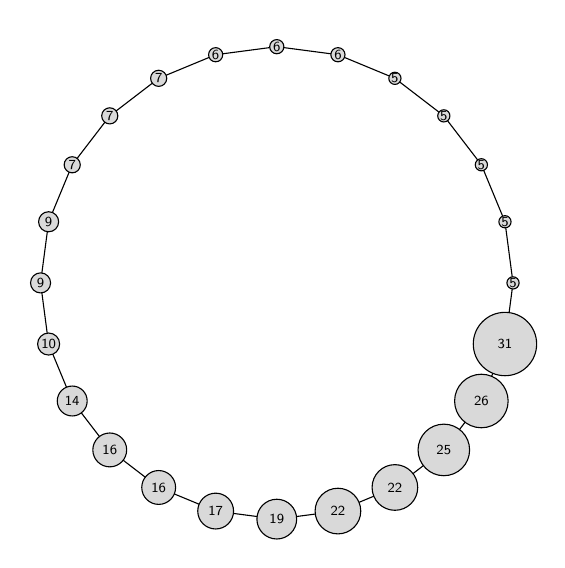
\begin{tikzpicture}
\def\cradius{3.0};
%\draw[help lines,step=1] (0,-5) grid (10,5);
\edef\counter{0};
%\def\sizes{{ 4, 4, 4, 9, 15, 17, 45, 52}};
\def\sizes{{5, 5, 5, 5, 5, 6, 6, 6, 7, 7, 7, 9, 9, 10, 14, 16, 16, 17, 19, 22, 22, 25, 26, 31}};

\draw (0:\cradius)
\foreach \x in {0,15,...,345}{ -- (\x:\cradius) }-- cycle (90:\cradius) node[above] {};

\foreach \angle in {0,15,...,345}{
      \def\cliquer{ {\angle * 0.002} };
      
      \pgfmathsetmacro{\pg}{\sizes[\counter]}; % set the macro pg with the current value of counter
      \counter
      \fill[draw, fill=gray!30] (\angle:\cradius) circle (\pg * 0.0125+0.015);
      %\draw[fill=gray!30] (\angle:\cradius) circle [radius=0.1];
      \node[black] at (\angle:3) {{\tiny $\mathsf{{\pg}}$}};
      \pgfmathparse{\counter + 1}; \xdef\counter{\pgfmathresult}; % increment counter and store the result again in counter
      }
\end{tikzpicture}
\caption{Power-law ring of cliques. Every circle is a complete graph (clique). Every clique is connected to its neighbors with one single link. The sizes of the cliques are randomly sampled from a power-law distribution with minimum clique size $\min_c=5$, maximum clique size $\max_c=75$, $n=150$, $\tau_c=1$.}
\label{fig:ring_of_clique_powerlaw}
\end{figure}

%%%%%%%%%%%%%%%%%%%%%%%%%%%%%%%%%%%%%%%%%%%%%%%%%%%%%%%%%%%%%%%%%%
%%%%%%%%%%%%%%%%%%%%%%%%%%%%%%%%%%%%%%%%%%%%%%%%%%%%%%%%%%%%%%%%%%

\subsection{Synthetic resting state networks}
Here we introduce a theoretically sound method for the generation of synthetic FC networks that mimic properties of resting state fMRI networks, including noise and intersubject variability, while presenting a pre-determined ground-truth modular structure against which the performance of community detection algorithms can be tested.

The general idea is that, starting from an adjacency matrix with a given modular structure, we can generate time-courses for each of the nodes whose pairwise correlations reproduce the edge structure of the original matrix. Noise can be added to the time-courses, and the resulting correlation matrix will provide a noisy representation of the original one. This procedure can be repeated multiple times to produce different datasets that represent different "subjects" in the study.

In practical terms, given an undirected weighted graph  $\mathbf{C} \in \mathbb{R}^{n\times n}$ whose community structure is known a-priori, we have calculated its nearest positive definite matrix~\cite{Higham1988} and its Cholesky decomposition, i.e. an upper triangular matrix $\mathbf{L}\in \mathbb{R}^{n\times n}$ such that $\mathbf{L}\mathbf{L}^T=\mathbf{C}$. Starting from uncorrelated variables $\mathbf{X} \in \mathbb{R}^{n \times l}$, we have generated correlated random variables $\mathbf{Y}=\mathbf{L} \mathbf{X}$ such that $\mathbb{E}(\mathbf{Y}\mathbf{Y}^T)=\mathbf{C}$. Additionally, we have injected different levels of noise into $\mathbf{Y}$ prior to the computation of the correlation matrix. 
\footnote{Since the covariance matrix of a zero-mean, unit-variance random variable $X$ is given by $\mathbb{E}(XX^T)$, it's easy to verify that $\mathbb{E}(YY^T)=\mathbb{E}(LX)(LX)^T=\mathbb{E}(LX)X^T L^T=L\mathbb{E}(XX^T)L^T=L^T\mathbf{I}L=C$} 
Schematic of this procedure is shown in Figure~\ref{fig:flowchart}.

We tested this idea on two different models of planted partition: a variant of the ring of cliques~\cite{fortunato2007} and the Lancichinetti-Fortunato-Radicchi (LFR) network~\cite{lancichinetti2008} (Figure \ref{fig:lfrringclique}, whose degree distribution and modular structure can be tuned to replicate topological features of real-world networks, including scale freeness~\cite{hagmann2008} and the presence of densely interconnected cores~\cite{vandenheuvel2011}.

\begin{sidewaysfigure}[htb!]
\centering
\includegraphics[height=0.25\textheight]{images/flowchart.pdf}
\caption{Flowchart of the generation and analysis of the synthetic datasets. In A the network with a pre-defined community structure is generated. The adjacency matrix is then processed in block B to obtain the nearest positive definite matrix for the Cholesky decomposition. This enables the generation of node-wise time-courses into which different levels of noise can be injected. The procedure is repeated multiple times to generate different instances (mimicking different subjects in the sample). Finally, correlation matrices are calculated for each instance (block C), and Fisher transformed to calculate the average adjacency matrix for analysis by community detection algorithms (block D). Lastly, resulting partitions are compared with the original, planted one in terms of NMI.}
\label{fig:flowchart}
\end{sidewaysfigure}

%%%%%%%%%%%%% COMPARING COMMUNITY STRUCTURE IN NETWORKS %%%%%%%%%%
\section{Comparing community structure in networks}
Some benchmark networks come with an annotated community structure representing the ground-truth assignment of nodes into communities, the annotations being made by experts in the field, like for example the karate club network of Zachary~\cite{zachary1977} or the political blog network~\cite{adamic2005}.
Moreover, generative models of networks like the stochastic block model and its variants, the planted partition model and the LFR benchmark, have a known ground-truth community.
As the number of community detection methods increased over the years, also a quantitative way to assess their performance was needed.

A large number of functions for comparing similarities and differences between partitions of a network have been proposed in the past.
They are used to provide quantitatively a number that tells how two partitions are similar.
Typically the result is normalized in the $[0,1]$ range, being towards $1$ for very similar clusterings and toward $0$ when mostly dissimilar.
These metrics are adopted especially in the benchmarking of community detection methods when the specific outcome of some algorithm is compared with a ground truth partition, usually, a-priori determined.

The most well-grounded and performing metrics for the comparison of two community structures are rooted in information theory~\cite{cover2006}.
The \emph{Normalized Mutual Information}~\cite{danon2005} and the \emph{Variation of Information}~\cite{meila2007} are the most widely used, despite it was recently found that both of them suffer of systematic errors due to the finite size of the network~\cite{zhang2015a}.
In the rest of the discussions, we ignore the limitation of finite size effects, by only working with relatively large networks.

Normalized Mutual Information (NMI) assumes that the clustering comparison is a problem of message decoding.
Implicit in this is the idea that if two partitions are similar, inferring one partition from the other needs very little information.
Let us consider two generic partitions of a graph denoted by their clusterings $\zeta^x,\zeta^y$ with $c_x$ and $c_y$ communities respectively: $\zeta^x=\{\zeta^x_1,\ldots,\zeta^x_{c_x}\}$ and $\zeta^y=\{\zeta^y_1,\ldots,\zeta^y_{c_y}\}$.
The number of nodes in the $i$-th community of $\zeta^x$ is $n_i :=|\zeta^x_i|$ and the number of nodes in the $j$-th community of $\zeta^y$ is $n_j:=|\zeta^y_j|$.
The two communities share a number of nodes $n_{ij}=| \zeta^x_i \cap \zeta^y_j|$.
Let us also consider the community assignments $\boldsymbol\sigma^x_i$ and $\boldsymbol\sigma^y_i$ for partitions $\zeta^x$ and $\zeta^y$ respectively; we treat the labels as values of two random variables $X$ and $Y$ with joint distribution $P(x,y)=P(X=x, Y=y) = n_{xy}/n$, which implies that $P(x)=P(X=x)=n_x^X/n$ and $P(y)=P(Y=y)=n_y^Y/n$.

The \emph{mutual information} between the two clusterings $\zeta^x,\zeta^y$ is then defined as $I(X,Y)=H(X) - H(X|Y)$ where $H(X)=-\sum_x p(x) \log p(x)$ is the Shannon entropy of $X$~\cite{cover2006}.
The mutual information itself is not very useful, because hierarchically splitting the clusters in $\zeta^x$ would produce no change in the prior $H(X|Y)$ and partitions with different hierarchies of the same clusters, would go unnoticed.
This observation led Danon~\cite{danon2005} to introduce normalized mutual information for clustering comparison as: 
\begin{equation}\label{eq:nmi}
\textrm{NMI}(X,Y) = \frac{2I(X,Y)}{H(X)+H(Y)} = \dfrac{2\sum \limits_{i=1}^{c_x} \sum \limits_{j=1}^{c_y} \frac{n_{ij}}{n} \log\left( \frac{n_{ij}n}{n_i n_j} \right)} {\left(-\sum \limits_{k=1}^{c_x} \frac{n_k}{n}\log\left(\frac{n_k}{n}\right) \right) + \left(-\sum \limits_{k=1}^{c_y} \frac{n_k}{n}\log\left(\frac{n_k}{n}\right) \right)}.
\end{equation}

Meila~\cite{meila2007} proposed another measure based on entropy, Variation of Information (VI), shown in Figure~\ref{fig:venn_diagram}.
VI measures how much knowing the cluster assignment for an item in clustering $X$ reduces the uncertainty about the item's cluster in clustering $Y$.
It's defined as:
\begin{equation}\label{eq:vi}
\textrm{VI}(X,Y) = H(X|Y) + H(Y|X)
\end{equation}
and it has the desirable property that, being a proper distance, it defines a metric on the space of the partitions.
Variation of information is also a local measure, i.e. the similarity of partitions differing only in a small portion of a graph depends on the differences of the clusters in that region, and not on the partition of the rest of the graph.
As noted by Karrer \cite{karrer2008} VI is upper-bounded by a $\log(n)$ factor, so a simple normalization brings it in the $[0,1]$ range.
Importantly, VI is zero for maximally equal partitions and $1$ for mostly dissimilar, inversely to NMI.
It's worth noting that the majority of the aforementioned metrics do not take in consideration comparison of pairs of communities between two partitions, but they insist on finding the overall similarity to summarize it in a single scalar.

\begin{figure}[htb!]
\centering
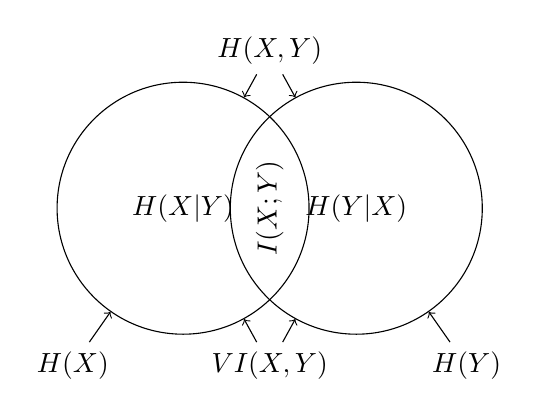
\begin{tikzpicture}
    \node[draw,circle,minimum size=3.2cm, inner sep=0cm] at (-1.1cm,0cm) (CL) {$H(X|Y)$};
    \node[draw,circle,minimum size=3.2cm, inner sep=0cm] at (1.1cm,0cm) (CR) {$H(Y|X)$};    
    \node[rotate=90] at (0cm,0cm) (IXY) {$I(X;Y)$};
    \node[] at (0cm,2cm) (HXY) {$H(X,Y)$};
    \node[] at (-2.5cm,-2cm) (HX) {$H(X)$};
    \node[] at (2.5cm,-2cm) (HY) {$H(Y)$};
    \node[] at (0cm,-2cm) (VI) {$VI(X,Y)$};
    \draw[->] (HX) -- (CL);
    \draw[->] (HY) -- (CR);
    \draw[->] (HXY) -- (CL);
    \draw[->] (HXY) -- (CR);
    \draw[->] (VI) -- (CL);
    \draw[->] (VI) -- (CR);
\end{tikzpicture}
\caption{Venn diagram representation of the important quantities used to treat the clustering comparison problem in terms of information theory.
The two circles are the entropies of variables $X$ and $Y$.
The mutual information $H(X;Y)$ is the intersection of the information in $X$ with the information in $Y$.
The Variation of information is equal to $VI(X;Y)=H(X|Y)+H(Y|X)=H(X)+H(Y)-2I(X;Y)$ because $I(X;Y)$ is counted twice.}
\label{fig:venn_diagram}
\end{figure}


It is also possible to quantify the confusion matrix $\mathbf{C}$ between the detected and planted modules.
Each element $C_{ij}$ is the number of nodes in the planted community-$i$ that appear in the detected community-$j$.
For each planted community one scores as true positives (TP) the nodes correctly identified as belonging to the ground-truth community, and as false positives (FP) the nodes wrongly assigned to a community; similarly false negatives (FN) are nodes wrongly classified in different communities and true negatives (TN) the nodes correctly classified as out of the community. Sensitivity, defined as $TP/(TP+FN)$, decreases with increasing number of False Negatives. Specificity instead is defined as $TN/(TN+FP)$ and decreases when many nodes are wrongly assigned in the same community. 

Accuracy (Acc) and Matthew Correlation Coefficient (MCC) are defined on the basis of the confusion matrix as:
\begin{align*}
\textrm{Acc}=\frac{(TP+TN)}{TP+FP+TN+FN} \qquad \textrm{MCC}=\frac{(TP\times TN-FP\times FN)}{\sqrt{(TP+FP)(TP+FN)(TN+FP)(TN+FN)}}
\end{align*}
where TP, TN, FP, FN are the number of true positives, true negatives, false positives and false negatives identified in the detected partition with respect to the planted partition.

Accuracy takes in account the proportion of correctly classified samples and can present relatively high values even in the case of poorly performing detection methods when the classes have very different size.
The Matthew Correlation Coefficient  takes into account true and false positives and negatives. It's a balanced coefficient, to use especially when classes are very imbalanced.


%%%%%%%%%%%%%%%%%%%%%%%%%%%%%%%%%%%%%%%%%%%%%%%%%%%%%%%%%%%%%
%%%%%%%%%%%%%%%%%%% PERCOLATION ANALYSIS %%%%%%%%%%%%%%%%%%%%
%%%%%%%%%%%%%%%%%%%%%%%%%%%%%%%%%%%%%%%%%%%%%%%%%%%%%%%%%%%%%
\section{Percolation analysis}\label{sec:percolation_analysis}
Functional connectivity networks are typically obtained as similarity matrices of physiological time signals over different brain areas.
The process of converting such similarity matrices into graphs, described in the previous chapters is not obvious.
In most of the works, a threshold is chosen such that all the edge weights greater than a given value are kept, while other links, indicative of correlations due to possibly noisy components are discarded.
Sparsification procedures are often applied to remove the weakest edges, which are the most affected by experimental noise, and to reduce the density of the graph, thus making it theoretically and computationally more tractable.
Indeed, weak links may contain significant structural information~\cite{thomas2011}, and procedures to identify the optimal trade-off are the subject of active investigations~\cite{zahoranszky-kohalmi2016a}.
The network can then be binarized, by setting all edge weights to unity.
Whether this sparsification procedure may help obtaining a better view on the underlying structure of networks, it represents an hot debate in the literature~\cite{rubinov2010,thomas2011}.
Ideally the obtained network should retain structural relations and ignore spurious links, but how is it possible to determine a proper value of threshold?
No well-accepted method to choose the best threshold has been adopted pragmatically in the brain networks literature and different scholars motivated their choice by different needs~\cite{gallos2012,lee2011,scheinost2012}.

As the final network density is of fundamental importance when performing community detection, the clustering outcome depends heavily on it.
Hence, a completely data-driven thresholding procedure is needed, that helps in transforming a similarity matrix into a network.


Percolation analysis, a method grounded in statistical physics, is suggested here as a method to identify the optimal sparsification threshold for community detection in brain connectivity networks.
The percolation threshold corresponds to the point where the largest connected component of the network starts breaking apart.
A threshold just below this point is the one that maximizes the information extracted by subsequent application of community detection algorithms, and has been applied and validated in human~\cite{gallos2012} and animal~\cite{bardella2016a} studies.

The most common choice when comparing networks from different groups, is to adopt a fixed threshold that keeps the same number of edges in the two groups.
This does not take in account the particularities of the analyzed group and datasets.
Percolation analysis should enable data-driven determination of the optimal sparsification threshold that preserves network structure and connectedness while removing potentially spurious correlations.
It is indeed important to stress that the distribution of the weight as well as the density or connectivity of the population are not exploited when using fixed thresholds and the final result does not mirror these information.
To this end, it has been demonstrated, especially in patient group such as in schizophrenia, autism or alcoholism, that the brain presents weaker connectivity than in health control persons~\cite{alexander-bloch2010}.

